\documentclass{article}
\usepackage[utf8]{inputenc}
\usepackage{titling}
\usepackage{graphicx}
\graphicspath{ {./img/} }

\newcommand{\subtitle}[1]{%
  \posttitle{%
    \par\end{center}
    \begin{center}\large#1\end{center}
    \vskip0.5em}%
}

\title{Capytaine: waves and floating bodies}
\subtitle{CMSC6950 Course Project - 2021 Spring}
\author{Ruixin Song, 202093805}
\date{June 16, 2021}

\begin{document}

\maketitle

\section{Introduction}
Capytaine\cite{Ancellin2019} is a python-based package reproduces an open-sourced software Nemoh, which is a Boundary Element Method (BEM) solver in the Computational Fluid Dynamics (CFD) domain. Applied to python, Capytaine reinforces the solver by utilizing the computational flexibility in python and combining with other efficient tools in the python scientific ecosystem such as VTK, NumPy, xarray, etc. \\

More specifically, Capytaine focuses on solving the problems of the water waves interacting with the floating bodies. It supports the computation of added mass, radiation damping, diffraction force and Froude-Krylov force for rigid bodies. For the theoretical part, it can perform Green Function and Kochin Function calculation inherited from Nemoh's core functionalities. Aside from these, Capytaine implemented 3D animation of the floating bodies motion and free surface elevation, which can function with the Visualization Toolkit (VTK).\\

With the features in Capytaine, the project defines several computational problems and uses the functionalities in the package to solve them, then extracts subset data from the results and makes them visible with Matplotlib and VTK.

\section{Computational tasks}
This project defines three computational tasks integrated in two separate scripts: \texttt{radiation.py} and \texttt{wave.py}. The following part is an overview for each computational task in the script.
\begin{enumerate}
    \item Task 1 in \texttt{radiation.py}\\
    Set radiation problems with different set of variables: water depth, liquid density, frequency, acceleration of gravity, and calculate the added mass and radiation damping for each variable group. 
    
    The goal of task1 is to find the trend of the added mass and radiation damping through the change of a single physical variable. In each processing unit, only change the target physical variable without modifying the others. For example, if we want to figure out how water depth will affect the added mass and radiation damping, we will keep default values for the other variables: water density, wave frequency and the gravity, etc.
    \item Task 2 in \texttt{wave.py}\\
    Set a diffraction problem with a sphere and a list of wave frequency. Solve the problem with the BEM solver and calculate the wave length, wave number and the wave period with different frequency values. The goal of task 2 is to find the correlation of the frequency, wave length, wave number and the period.
    \item Task 3 in \texttt{wave.py}\\
    Generate the second geometry: a cylinder, along with the sphere in Task2. Calculate the influence matrices between the two floating bodies with customized green function. The goal of task3 is to see how one floating body might affect the other when they are positioned closely.
\end{enumerate}
After defining the computational tasks, we should be able to explore in the Capytaine package to find the solutions.

\section{Solutions}
Capytaine has several functionalities to address the computational tasks we have defined in section2. Here introduce these functions and explain how they address our issues.
\begin{enumerate}
    \item \texttt{RadiationProblem()} and \texttt{DiffractionProblem()}\\
    The two problem functions in Capytaine are derived from the LinearPotentialFlowProblem class, help to define the computational fluid problems. The parameters in the functions involving free surface, sea bottom, wave frequency, acceleration of gravity, have default values complied to the environment in Earth that can be applied to most of the computational cases. \\
    In task1, the series of problems are set by \texttt{RadiationProblem()}, with modifying the parameter groups. I customized 4 variable groups: a list of water depth(sea bottom), a list of omega (wave frequency), a list of g (acceleration of gravity), and a list of rho (liquid density). When performing the computation for each group, the remaining parameters in the problem function are kept with default values. \\
    In task2, I defined the problem by the \texttt{DiffractionProblem()} since I want to explore the diffraction force and Froude-Krylov force features in it. But things are not going smoothly, the computation result of diffraction force and Froude-Krylov force are stored in complex128 data format, that is performed in complex numbers. Without background in hydro-mechanics, I was not be able to figure out how to deal with the two kinds of forces in complex numbers. Therefore, I simplified the problem to retrieve the calculation results of wave period, wave length and wave number, after using the problem solver \texttt{BEMSolver()}.
    \item \texttt{BEMSolver()} and \texttt{HierarchicalToeplitzMatrixEngine()}\\
    Derived from Nemoh, the \texttt{BEMSolver()} in Capytaine is a solver for BEM problems. It has two parameters: green function and engine type, which can be customized by users. In my computational tasks1 and task2, I use the \texttt{BEMSolver()} with the \texttt{HierarchicalToeplitzMatrixEngine()} instead of the default \texttt{BasicMatrixEngine()}. After calculation, the solver function will return an Xarray data set, in which all the parameters and calculation results are inclusive.
    \item \texttt{engine.build\char`_matrices()}\\
    The \texttt{build\char`_matrices()} feature in the \texttt{engine} class can perform the calculation of influence matrices of two given floating body meshes. The important parameters need to be set when calling the \texttt{build\char`_matrices()} are two mesh objects and the green function. In task3, I use a \texttt{BasicMatrixEngine()} and call the \texttt{build\char`_matrices()} function with the two floating body objects "sphere" and "cylinder" to calculate the influence matrices. After processing, the function returns two matrices S and K.
\end{enumerate}
After the solutions complete the computational tasks, the results can be assembled by the \texttt{assemble\char`_dataset()} function in Capytaine, which produces an Xarray data set. Then these Xarray data sets can be saved as NetCDF format files and passed to the visualization tasks. For the complex number in the computation results, for example the diffraction forces after performing solution to \texttt{DiffractionProblem()}, can use \texttt{separate\char`_complex\char`_values} in the \texttt{capytaine.io.xarray} module.

\section{Visualization}
All the visualization work are doing in the scripts \texttt{plot\char`_radiation.py} and \texttt{plot\char`_wave.py}. The following part will explain the data showing in each plot.
\begin{enumerate}
    \item Derived from the computation task1, figure \ref{fig:plt1} displays the variation of added mass and the radiation damping with each of the variable groups. The corresponding code can be found in the \texttt{plot\char`_radiation.py}. From the plotting result, we may find the trend of the added mass and radiation damping with the growth of water depth, liquid density, wave frequency and the acceleration of gravity.
    \begin{figure}[ht]
        \centering
        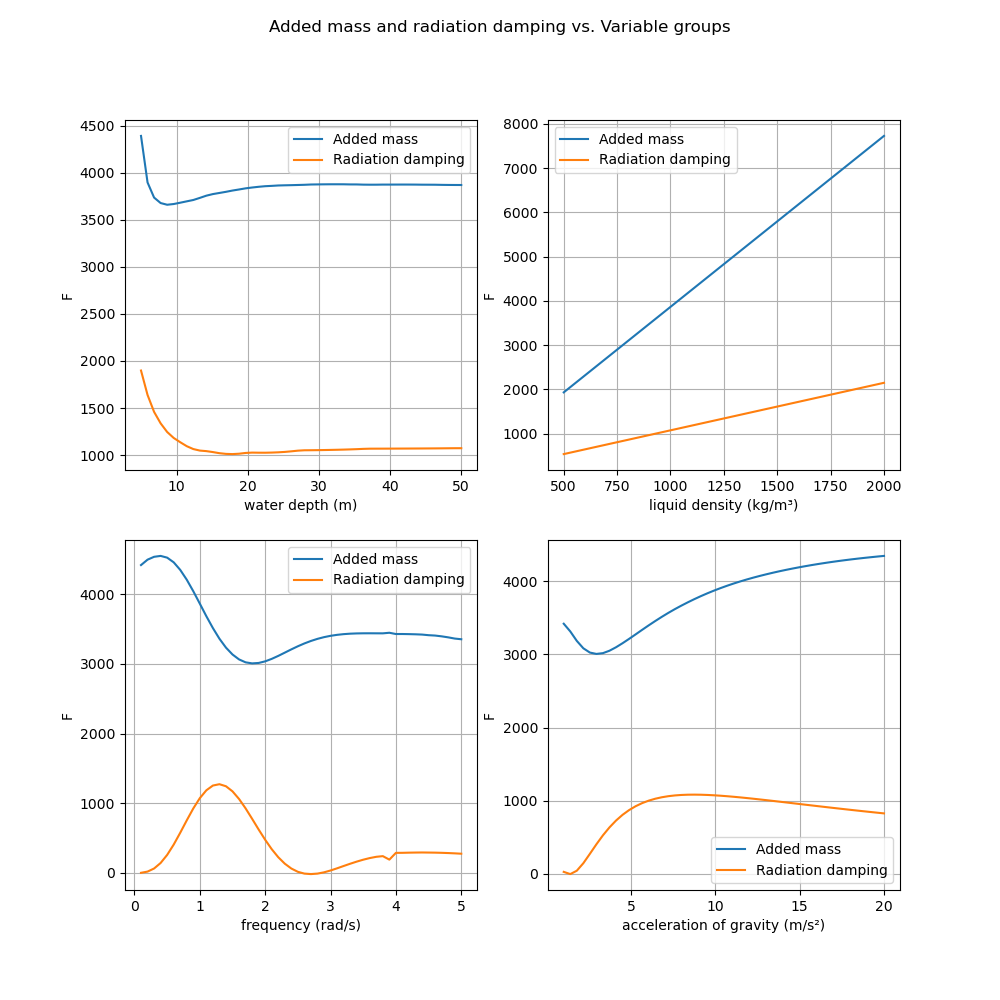
\includegraphics[width=1\textwidth]{img/1_radiation.png}
        \caption{added mass and radiation damping}
        \label{fig:plt1}
    \end{figure}
    \item Figure \ref{fig:plt2} from computational task2 plots the correlation of wave numbers, wave frequency, wave length and wave period. From the plot we may easily find the wave number is positively correlated with wave frequency, and negatively correlated with wave period and wave length. The corresponding code can be found in the script \texttt{plot\char`_wave.py}. The detailed plot can be viewed in Matplotlib by rotating the plot object.
    \begin{figure}[ht]
        \centering
        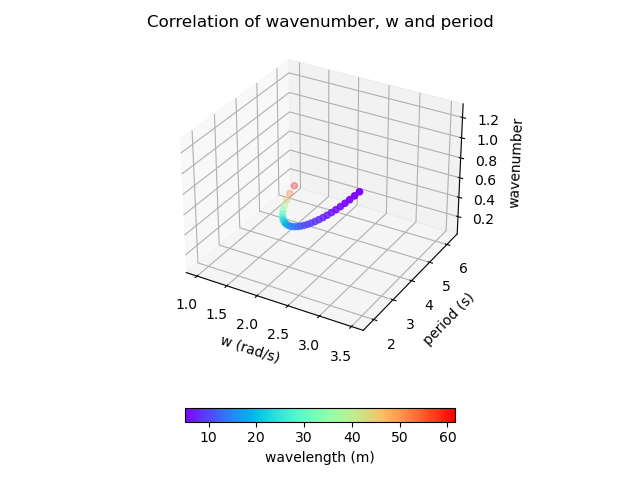
\includegraphics[width=1\textwidth]{img/2_1_correlation.png}
        \caption{Correlation of wavenumber, frequency, wavelength and period}
        \label{fig:plt2}
    \end{figure}
    \item The data used in figure \ref{fig:plt3} is a subset of results in task2, the wave frequency. In the original plan, I want to use the free surface elevation data to generate the contour plot. However the data in the elevation array is one-dimension and hard to decoded in Matplotlib since they are values matching with the free surface normal. Therefore, I use sine() function to simulate the water waves, but some defect exists: the real wave amplitude decays with propagation distance, and this part might be fixed with exponent function. 
    \begin{figure}[ht]
        \centering
        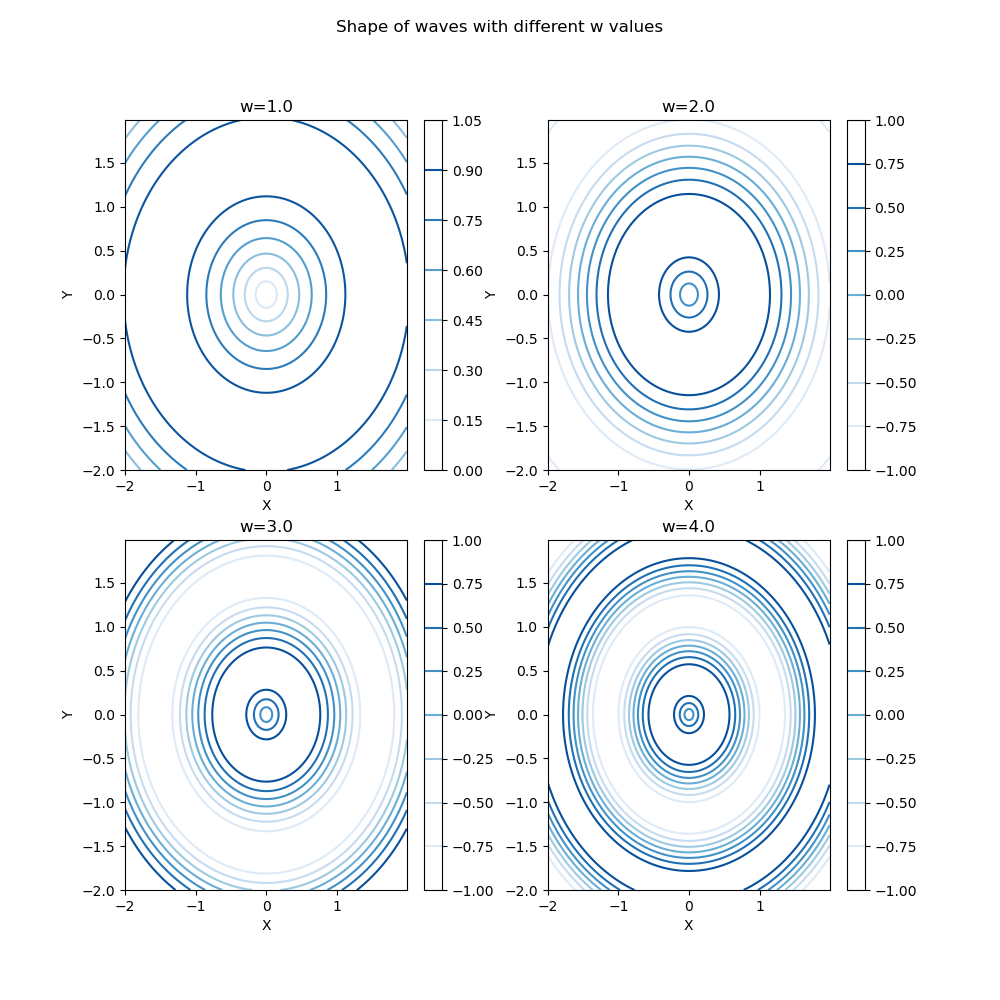
\includegraphics[width=1\textwidth]{img/2_2_waveshape.png}
        \caption{Wave shapes with different wave frequency}
        \label{fig:plt3}
    \end{figure}
    \item Figure \ref{fig:plt4} depict the influence matrices of two floating bodies, which is derived from the computational task3. The matrices are not square because the given mesh sizes are different. The corresponding code can be found in \texttt{plot\char`_wave.py}
    \begin{figure}[ht]
        \centering
        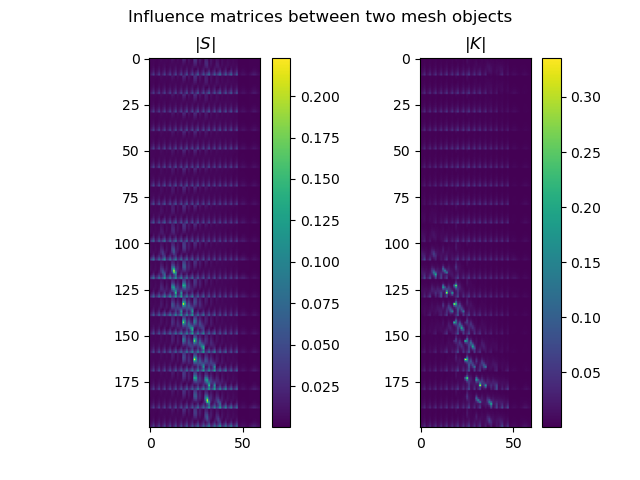
\includegraphics[width=1\textwidth]{img/2_3_infmatrix.png}
        \caption{Influence matrices of two floating bodies}
        \label{fig:plt4}
    \end{figure}

\end{enumerate}

\section{Workflow I/O}
Figure \ref{fig:plt5} depicts the workflow of the project.
\begin{figure}[ht]
    \centering
    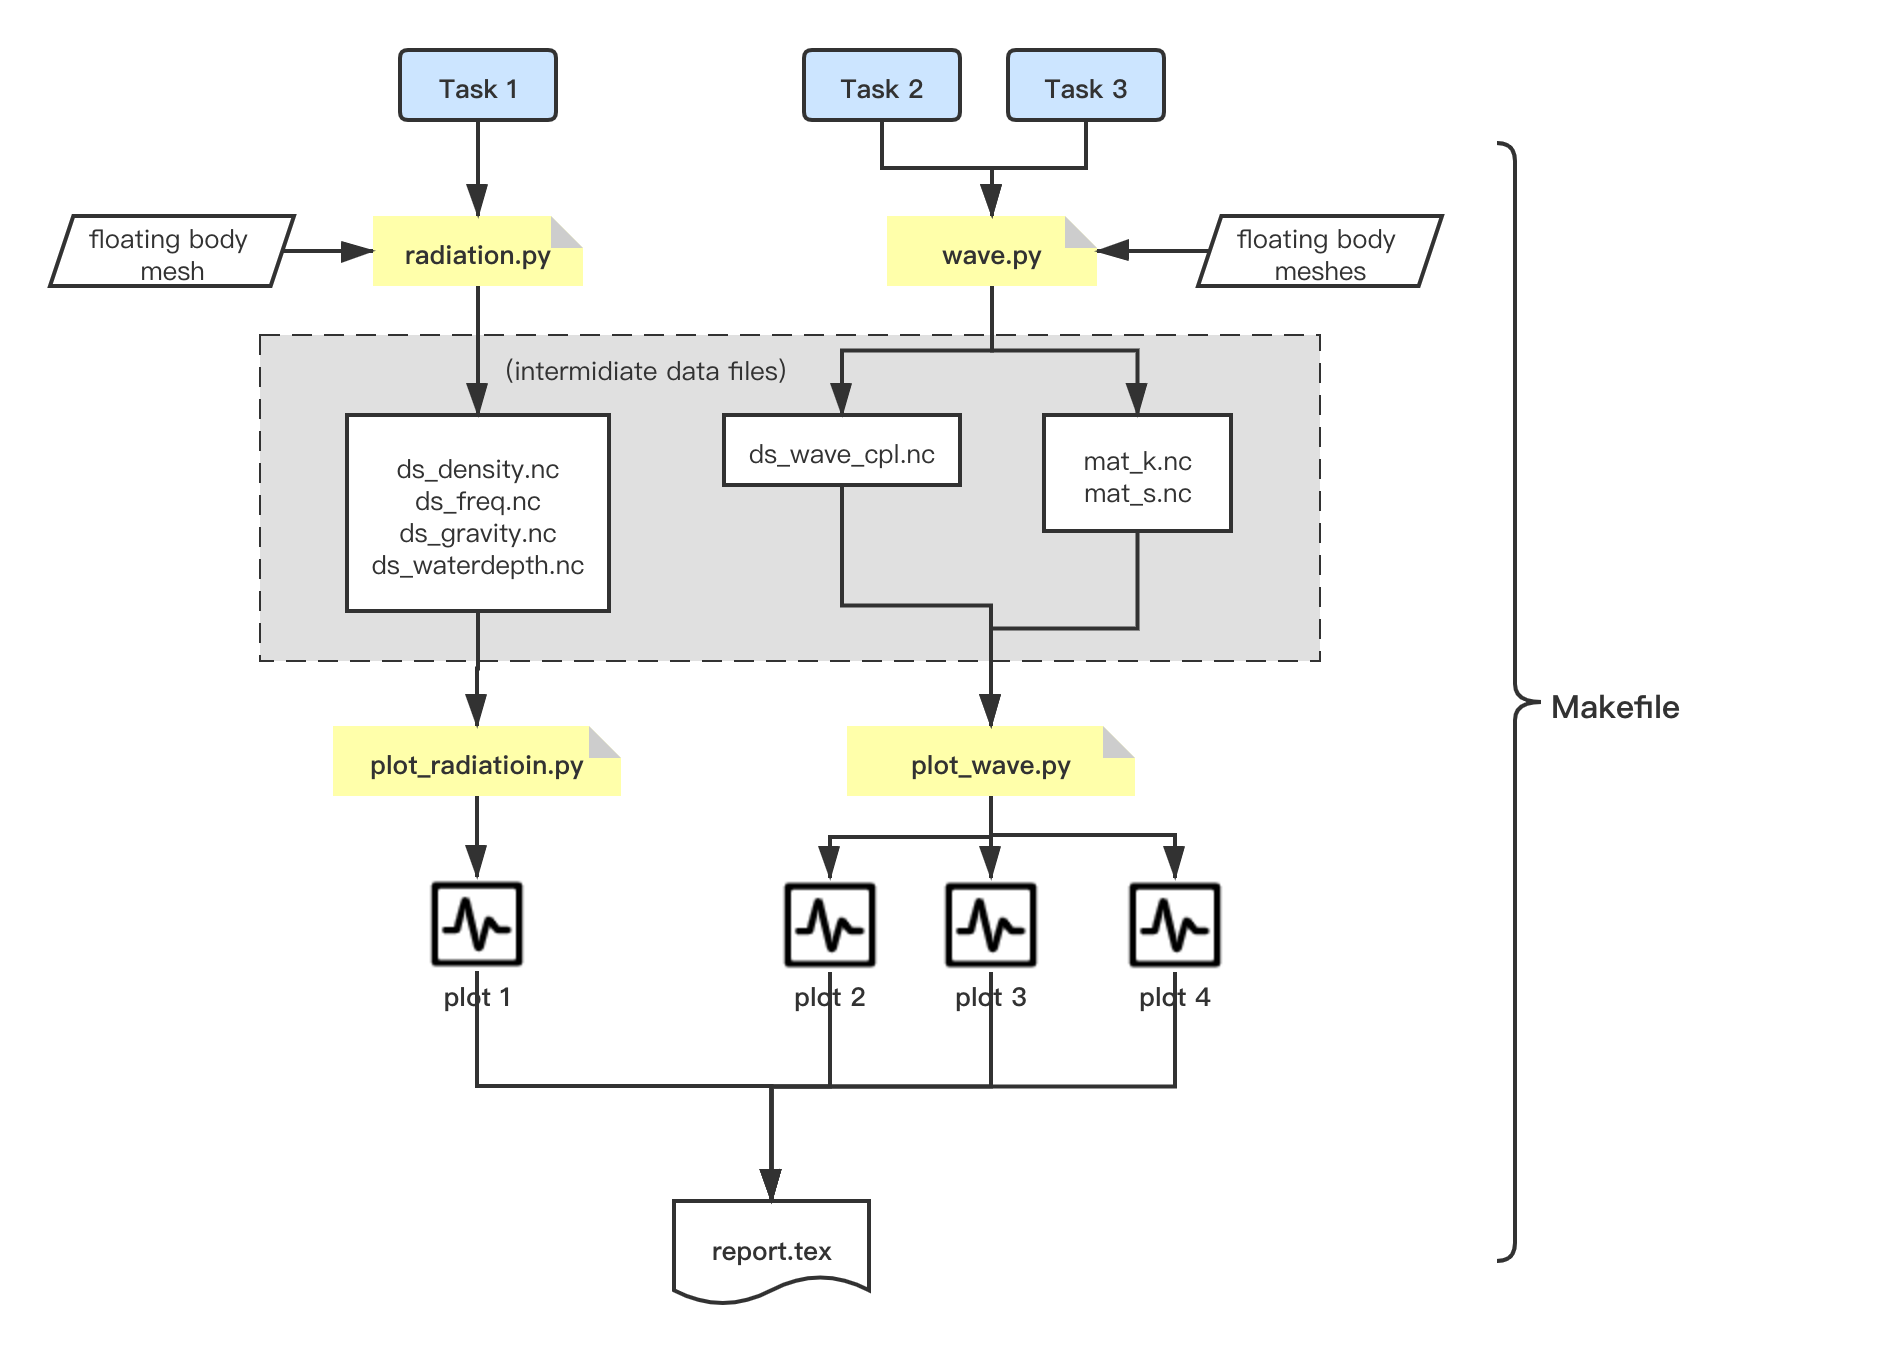
\includegraphics[width=1.2\textwidth]{workflow.png}
    \caption{workflow of the project}
    \label{fig:plt5}
\end{figure}

\clearpage
\bibliographystyle{ieeetr}
\bibliography{ref}

\end{document}